
\documentclass[twoside,12pt]{article}
%\documentclass[UTF8]{ctexart}
\usepackage[heading=true]{ctex}

\RequirePackage{natbib}
% modification to natbib citations
\setcitestyle{authoryear,round,citesep={;},aysep={,},yysep={;}}

\usepackage{booktabs}
\usepackage{threeparttable}
\usepackage{multirow}

\usepackage{listings}
\usepackage{color}

\definecolor{dkgreen}{rgb}{0,0.6,0}
\definecolor{gray}{rgb}{0.5,0.5,0.5}
\definecolor{mauve}{rgb}{0.58,0,0.82}

\lstset{frame=tb,
  language=Python,
  aboveskip=3mm,
  belowskip=3mm,
  showstringspaces=false,
  columns=flexible,
  basicstyle={\small\ttfamily},
  numbers=none,
  numberstyle=\tiny\color{gray},
  keywordstyle=\color{blue},
  commentstyle=\color{dkgreen},
  stringstyle=\color{mauve},
  breaklines=true,
  breakatwhitespace=true,
  tabsize=3
}

\usepackage{fancyhdr} % 页眉页脚
\usepackage{graphicx}
\usepackage{amsmath}
\usepackage[colorlinks=true, allcolors=blue]{hyperref}
\usepackage{geometry}

\geometry{
  paper      = a4paper,
  vmargin    = 2.54cm,
  hmargin    = 3.17cm,
  headheight = 0.75cm,
  headsep    = 0.29cm,
  footskip   = 0.79cm,
}

\newcommand{\update}[1]{{\textcolor{black}{#1}}}
\newcommand{\boldres}[1]{{\textbf{\textcolor{red}{#1}}}}
\newcommand{\secondres}[1]{{\underline{\textcolor{blue}{#1}}}}

\pagestyle{fancy}

%\firstpageno{1}

\title{ }

\author{罗浩铭\ PB21030838}


\begin{document}

\fancyhf{} % 清除所有页眉页脚
\fancyfoot[C]{\thepage} % 设置右页脚为页码
\fancyhead[l]{\footnotesize  }
% 设置右页眉为章节标题 

\renewcommand{\headrulewidth}{0pt} % 去页眉线

\begin{center}
  \textbf{\LARGE{深度学习实践大作业——iTransformer}}\\
  \vspace{0.2cm}
  \large{罗浩铭\ PB21030838}
\end{center}
% 无错别字,语句通顺,格式整齐,排版良好  (5分)

\section{文章基本信息}

\begin{itemize}
  \item 论文题目:iTransformer: Inverted Transformers Are Effective for Time Series Forecasting~\citep{itransformer}
  \item 论文作者:Yong Liu, Tengge Hu, Haoran Zhang, Haixu Wu, Shiyu Wang, Lintao Ma, Mingsheng Long
  \item 论文来源:ICLR 2024(在投,但在OpenReview已经拿到3个8分和一个6分,基本确定中会,参见https://openreview.net/forum?id=JePfAI8fah)
  \item 首发日期:2023年10月10日
  \item 论文链接:\url{https://arxiv.org/abs/2310.06625}
  \item 论文官方实现:\url{https://github.com/thuml/iTransformer}(截至本报告完成时,已获得443颗星)
\end{itemize}



\section{文章介绍及理解}
% 简述对文章的理解   300-600字     (10分)

本文提出的iTransformer,即inverted Transformer,是一种新的基于Transformer~\citep{Transformer}的时间序列预测架构,它的做法其实非常简单:传统的Transformer架构是将同一时间点的各变量建模为一个token (temporal token),对变量维进行FFN计算,并对时间轴进行attention计算;而iTransformer则是将同一变量的序列建模为一个token (variate token),对时间维进行FFN计算提取时序特征,并对变量轴进行attention计算从而提取各变量之间的关联。也就是说,它倒置了传统Transformer架构中对时间轴和变量轴的处理方式,这也是其名字由来。正是这样的简单改进,使得其在不修改任何底层模块的条件下,大幅提升了模型性能,使之在各大复杂时序预测任务中取得了大幅领先的SOTA效果。

虽然其做法简单,但是其背后蕴含着深刻的思想。

首先,我们先来看传统Transformer架构的预测器为何表现不佳:
\begin{itemize}
  \item 一般而言,不同的变量具有完全不同的物理含义,即使语义相同,其度量单位也可能完全不同。此外,由于测量延迟等原因,其实际产生的时刻并不一定是严格对齐的。由此,同一时刻的多个变量服从不同的分布,且可能带时间偏移,作为token缺乏语义,容易学到无意义的注意力图
  \item 原本独立的变量在该架构下被杂糅为无法区分的特征通道,这会提高学习变量之间关联信息的难度
  \item 每个特征表示只能反映一个时间戳的特征,感受野过小;模型处理长期序列输入时,由于$O(n^2)$的attention计算复杂度,计算开销大,并且随着历史观新测的输入变长,预测效果反而下降
\end{itemize}

而iTransformer架构的好处在于:
\begin{itemize}
  \item 自注意力模块在其中能十分自然地提取到变量之间的关联信息,从而更好地捕捉变量之间的相互作用机制。
  \item 由于时间特征通常有着不少类似的模式,FFN适合提取时间特征,并有助于提高模型的泛化性
  \item Transformer中的层归一化(LayerNorm)可以帮助消除变量之间分布差异。
  \item 由于该架构只是改变了Transformer模型的用法,因此该工作可拓展到任意的魔改Transformer架构上,适用性极广。
\end{itemize}

由此,iTransformer架构在不修改任何底层模块的条件下,大幅提升了模型性能,并成为不少架构改进的新思路。

\section{代码结构}
% 对代码结构进行描述 300-1000字    (10分)

代码的总体结构为:以\verb |run.py|为入口,其拉起experiments部分中的主类,主类再调用data\_provider、model(model再调用layers)、utils等部分的类,完成数据的读取、模型的构建、训练、测试等过程。

下面自顶向底分别介绍代码的各部分:
\begin{itemize}
  \item script: 用于运行训练和测试的脚本,其中定义好了论文里的各个实验的脚本代码,特别是提供了合适的训练参数,可以直接运行。
  \item \verb |run.py|:整个程序的入口,用于接收命令行参数,并根据命令行参数,选择合适的实验类(是否是测试从部分变量的序列预测出全部变量的序列的实验),初始化后调用其训练、测试或预测函数,完成该次实验内容。
  \item model: 里面定义了Transformer, iTransformer,以及Transformer变体(包括Reformer~\citep{kitaev2020reformer}, Informer~\citep{Informer}, Flowformer~\citep{wu2022flowformer}, Flashformer~\citep{dao2022flashattention})及其inverted版本。
  \item layers: 包含上述模型中的各个子模块,如attention及其各种改型, FFN, encoder, decoder, embedding (含原版的embedding方案和inverted的方案)等。
  \item data\_provider: 用于根据实验配置信息,读取各个数据集的数据,并提供相应的Data Loader。
  \item utils: 包含各种工具函数和类,如计算各种评价指标、loss的函数,提供attention mask的类、时间序列处理工具类及工具函数、学习率调节、早停等。
\end{itemize}

从Transformer到iTransformer的改动相当简单,只需要将Embedding层由\verb |DataEmbedding|换为\verb |DataEmbedding_inverted|,并相应地用permute调换维度,调整维度大小即可。

\section{训练及测试过程}
% 对训练和测试过程进行描述(各种超参),需含loss曲线的展示,对时间的描述等   500-1000字	(15分)

本次作业中,我使用了iTransformer的官方实现\url{https://github.com/thuml/iTransformer}来进行复现。代码在软件工程规范上做得很好,模块化程度高,API设计合理,使用和修改都十分方便,读起来也赏心悦目。由于代码提供了bash脚本,里面指定了各个数据集的测试配置及超参设置,因此我们可以很方便地对论文中结果进行复现。

我们同时使用百度的aistudio(每日4小时额度,单卡V100)和kaggle平台(每周30小时额度,单卡P100)进行训练。总共花费了大约40小时额度的算力来完成下面所述的全部测试。

我们先用论文中提到的各数据集对iTransformer进行了测试,并将测试结果与原论文中的结果进行对比。测试所用数据集列表如表\ref{tab:dataset}所示。

此后,我们对比了iTransformer与Transformer的性能,测试了iFlashTransformer的效率提升,以及对各种超参进行了测试。

\begin{table}[thbp]
  \centering
  \vspace{0pt}
  \caption{\small{数据集描述,\emph{Dim}代表时间序列变量数,\emph{Dataset Size}以 (Train, Validation, Test)的形式表示,\emph{Prediction Length}表示各预测序列长度的设定,\emph{Frequency} 表示时间序列的采样时间间隔}\label{tab:dataset}}
  \vskip 0.15in
  \resizebox{\textwidth}{!}
  {
    \begin{threeparttable}
      \begin{small}
        \renewcommand{\multirowsetup}{\centering}
        \setlength{\tabcolsep}{4.5pt}
        \begin{tabular}{l|c|c|c|c|c}
          \toprule
          Dataset               & Dim & Prediction Length                     & Dataset Size                          & Frequency & Information                    \\
          \toprule
          \update{ETTh1, ETTh2} & 7   & \scalebox{0.8}{\{96, 192, 336, 720\}} & \scalebox{0.8}{(8545, 2881, 2881)}    & Hourly    & \scalebox{1.0}{Electricity}    \\
          \midrule
          \update{ETTm1, ETTm2} & 7   & \scalebox{0.8}{\{96, 192, 336, 720\}} & \scalebox{0.8}{(34465, 11521, 11521)} & 15min     & \scalebox{1.0}{Electricity}    \\
          \midrule
          \update{Exchange}     & 8   & \scalebox{0.8}{\{96, 192, 336, 720\}} & \scalebox{0.8}{(5120, 665, 1422)}     & Daily     & \scalebox{1.0}{Economy}        \\
          \midrule
          Weather               & 21  & \scalebox{0.8}{\{96, 192, 336, 720\}} & \scalebox{0.8}{(36792, 5271, 10540)}  & 10min     & \scalebox{1.0}{Weather}        \\
          \midrule
          ECL                   & 321 & \scalebox{0.8}{\{96, 192, 336, 720\}} & \scalebox{0.8}{(18317, 2633, 5261)}   & Hourly    & \scalebox{1.0}{Electricity}    \\
          \midrule
          Traffic               & 862 & \scalebox{0.8}{\{96, 192, 336, 720\}} & \scalebox{0.8}{(12185, 1757, 3509)}   & Hourly    & \scalebox{1.0}{Transportation} \\
          \midrule
          Solar-Energy          & 137 & \scalebox{0.8}{\{96, 192, 336, 720\}} & \scalebox{0.8}{(36601, 5161, 10417)}  & 10min     & \scalebox{1.0}{Energy}         \\
          \midrule
          \update{PEMS03}       & 358 & \scalebox{0.8}{\{12, 24, 48, 96\}}    & \scalebox{0.8}{(15617,5135,5135)}     & 5min      & \scalebox{1.0}{Transportation} \\
          \midrule
          \update{PEMS04}       & 307 & \scalebox{0.8}{\{12, 24, 48, 96\}}    & \scalebox{0.8}{(10172,3375,281)}      & 5min      & \scalebox{1.0}{Transportation} \\
          \midrule
          \update{PEMS07}       & 883 & \scalebox{0.8}{\{12, 24, 48, 96\}}    & \scalebox{0.8}{(16911,5622,468)}      & 5min      & \scalebox{1.0}{Transportation} \\
          \midrule
          \update{PEMS08}       & 170 & \scalebox{0.8}{\{12, 24, 48, 96\}}    & \scalebox{0.8}{(10690,3548,265)}      & 5min      & \scalebox{1.0}{Transportation} \\
          \bottomrule
        \end{tabular}
      \end{small}
    \end{threeparttable}
  }
  \vspace{0pt}
\end{table}

我们以Weather数据集下输入96长度序列并输出96长度预测序列的任务为例(见表\ref{tab:hyperparams})介绍我们训练时用的超参:
\begin{table}[htbp]
  \caption{\small{典型的训练超参设置(以Weather数据集下输入96长度序列并输出96长度预测序列的任务为例)}}
  \label{tab:hyperparams}
  \vspace{5pt}
  \centering
  \begin{tabular}{ccc}
    \toprule
    超参名称      & 解释              & 超参值 \\
    \midrule
    enc\_layers   & Encoder层数       & 3      \\
    dec\_layers   & Decoder层数       & 1      \\
    n\_heads      & 多头注意力头数    & 8      \\
    enc\_in       & Encoder输入变量数 & 21     \\
    dec\_in       & Decoder输入变量数 & 21     \\
    c\_out        & 输出变量数        & 21     \\
    d\_model      & Token维度         & 512    \\
    d\_ff         & FFN维度           & 512    \\
    batch\_size   & Batch大小         & 128    \\
    train\_epochs & Epoch数           & 10     \\
    lr            & 学习率            & 0.0001 \\
    \bottomrule
  \end{tabular}
\end{table}
由于Weather数据集较小,因此我们选用的Encoder层数仅为2,由于时间序列预测任务不需要很复杂的Decoder,因此Decoder层数仅为1。Encoder, Decoder输入变量数以及输出变量数与数据集保持一致即可。Token维度和FFN维度的设置默认如上。由于Weather数据集较小,单卡可以支持128的BatchSize,Epoch数为10,此类较大的模型学习率一般都设为0.0001。

我们以Traffic数据集下输入96长度序列并输出96长度预测序列的任务为例(因其未早停),来展示典型的训练过程中的每个epoch的loss曲线(见图\ref{fig:loss}):
\begin{figure}[htbp]
  \centering
  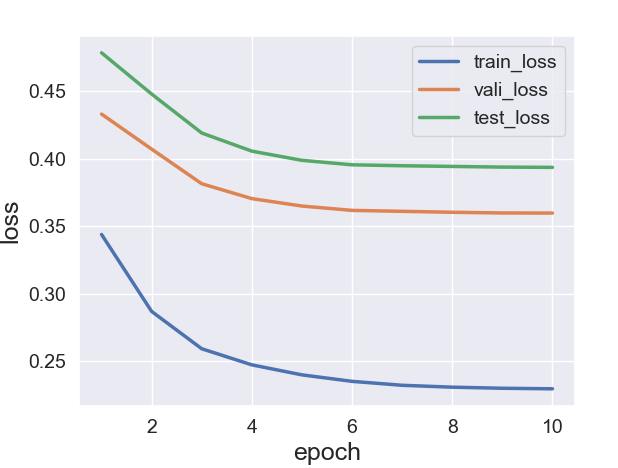
\includegraphics[width=0.8\textwidth]{./pic/loss_plot.png}
  \caption{\small{典型的训练过程中的loss曲线(以Traffic数据集下输入96长度序列并输出96长度预测序列的任务为例)}}
  \label{fig:loss}
\end{figure}

可以看到,训练过程中,不管是training loss, validation loss或者是test loss曲线,它们都呈现下降趋势,并 最终接近收敛。

在各个数据集中,取预测长度为96时(预测长度对训练时长有少许影响,但非主要因素),每个epoch的训练时长如表\ref{tab:time}所示:
\begin{table}[htbp]
  \caption{\small{各数据集下预测长度为96时每个epoch的训练时长}}
  \label{tab:time}
  \vspace{5pt}
  \centering
  \begin{tabular}{ccc}
    \toprule
    数据集       & 训练时长/epoch \\
    \midrule
    ETTm1        & 12s            \\
    ETTm2        & 12s            \\
    ETTh1        & 3s             \\
    ETTh2        & 3s             \\
    PEMS03       & 68s            \\
    PEMS04       & 89s            \\
    PEMS07       & 237s           \\
    PEMS08       & 22s            \\
    ECL          & 57s            \\
    Exchange     & 5s             \\
    Traffic      & 101s           \\
    Weather      & 34s            \\
    Solar-Energy & 31s            \\
    \bottomrule
  \end{tabular}
\end{table}
而每次训练最多需要十个epoch,因此在各数据集上的训练时间在半分钟到半小时不等。

\newpage
\section{复现结果}
% 复现结果与文章所示结果的对比,并分析结果不同的可能的原因  500-1000字    (15分)
\subsection{模型效果测试}
我们对论文中的所有数据集进行了测试,并将测试结果与原论文中的结果进行对比。测试结果如表\ref{tab:result}所示。

\newpage

\begin{table}[htbp]
  \caption{\small{复现结果与原论文结果对比(平均结果指四种预测长度的结果取平均)}}
  \label{tab:result}
  \vspace{5pt}
  \centering
  \resizebox{\textwidth}{!}
  {
    \begin{small}
      \renewcommand{\multirowsetup}{\centering}
      \setlength{\tabcolsep}{5.3pt}
      \begin{tabular}{c|c|cc|cc|cc|cc|cc}
        \toprule
        \multirow{2}{*}{Models}                                  & Prediction & \multicolumn{2}{c|}{ECL} & \multicolumn{2}{c|}{Exchange} & \multicolumn{2}{c|}{Traffic} & \multicolumn{2}{c|}{Weather} & \multicolumn{2}{c}{Solar-Energy}                                         \\
        \cmidrule(lr){3-4} \cmidrule(lr){5-6} \cmidrule(lr){7-8} \cmidrule(lr){9-10} \cmidrule(lr){11-12}
                                                                 & Length     & MSE                      & MAE                           & MSE                          & MAE                          & MSE                              & MAE   & MSE   & MAE   & MSE   & MAE   \\
        \midrule
        \multirow{5}{*}{\textbf{iTransformer (Our Replication)}} & 96         & 0.147                    & 0.239                         & 0.086                        & 0.206                        & 0.393                            & 0.269 & 0.176 & 0.216 & 0.208 & 0.243 \\
                                                                 & 192        & 0.168                    & 0.259                         & 0.180                        & 0.304                        & 0.413                            & 0.277 & 0.225 & 0.257 & 0.239 & 0.263 \\
                                                                 & 336        & 0.178                    & 0.270                         & 0.338                        & 0.422                        & 0.425                            & 0.283 & 0.281 & 0.299 & 0.251 & 0.275 \\
                                                                 & 720        & 0.210                    & 0.300                         & 0.853                        & 0.696                        & 0.459                            & 0.299 & 0.358 & 0.350 & 0.250 & 0.276 \\
        \cmidrule(lr){2-12}
                                                                 & Avg        & 0.176                    & 0.267                         & 0.364                        & 0.407                        & 0.423                            & 0.282 & 0.260 & 0.281 & 0.239 & 0.264 \\
        \midrule
        \multirow{5}{*}{\textbf{iTransformer}}                   & 96         & 0.148                    & 0.240                         & 0.086                        & 0.206                        & 0.395                            & 0.268 & 0.174 & 0.214 & 0.203 & 0.237 \\
                                                                 & 192        & 0.162                    & 0.253                         & 0.177                        & 0.299                        & 0.417                            & 0.276 & 0.221 & 0.254 & 0.233 & 0.261 \\
                                                                 & 336        & 0.178                    & 0.269                         & 0.331                        & 0.417                        & 0.433                            & 0.283 & 0.278 & 0.296 & 0.248 & 0.273 \\
                                                                 & 720        & 0.225                    & 0.317                         & 0.847                        & 0.691                        & 0.467                            & 0.302 & 0.358 & 0.349 & 0.249 & 0.275 \\
        \cmidrule(lr){2-12}
                                                                 & Avg        & 0.178                    & 0.270                         & 0.360                        & 0.403                        & 0.428                            & 0.282 & 0.258 & 0.279 & 0.233 & 0.262 \\
        \bottomrule
      \end{tabular}
    \end{small}
  }
  \resizebox{0.9\textwidth}{!}
  {
    \begin{small}
      \renewcommand{\multirowsetup}{\centering}
      \setlength{\tabcolsep}{5.3pt}
      \begin{tabular}{c|c|cc|cc|cc|cc}
        \toprule
        \multirow{2}{*}{Models}                                  & Prediction & \multicolumn{2}{c|}{ETTm1} & \multicolumn{2}{c|}{ETTm2} & \multicolumn{2}{c|}{ETTh1} & \multicolumn{2}{c}{ETTh2}                                 \\
        \cmidrule(lr){3-4} \cmidrule(lr){5-6} \cmidrule(lr){7-8} \cmidrule(lr){9-10}
                                                                 & Length     & MSE                        & MAE                        & MSE                        & MAE                        & MSE   & MAE   & MSE   & MAE   \\
        \midrule
        \multirow{5}{*}{\textbf{iTransformer (Our Replication)}} & 96         & 0.342                      & 0.377                      & 0.186                      & 0.272                      & 0.387 & 0.405 & 0.301 & 0.350 \\
                                                                 & 192        & 0.383                      & 0.396                      & 0.254                      & 0.314                      & 0.441 & 0.436 & 0.380 & 0.399 \\
                                                                 & 336        & 0.418                      & 0.418                      & 0.316                      & 0.351                      & 0.491 & 0.462 & 0.424 & 0.432 \\
                                                                 & 720        & 0.487                      & 0.457                      & 0.414                      & 0.407                      & 0.509 & 0.494 & 0.430 & 0.447 \\
        \cmidrule(lr){2-10}
                                                                 & Avg        & 0.408                      & 0.412                      & 0.293                      & 0.336                      & 0.457 & 0.449 & 0.384 & 0.407 \\
        \midrule
        \multirow{5}{*}{\textbf{iTransformer}}                   & 96         & 0.334                      & 0.368                      & 0.180                      & 0.264                      & 0.386 & 0.405 & 0.297 & 0.349 \\
                                                                 & 192        & 0.377                      & 0.391                      & 0.250                      & 0.309                      & 0.441 & 0.436 & 0.380 & 0.400 \\
                                                                 & 336        & 0.426                      & 0.420                      & 0.311                      & 0.348                      & 0.487 & 0.458 & 0.428 & 0.432 \\
                                                                 & 720        & 0.491                      & 0.459                      & 0.412                      & 0.407                      & 0.503 & 0.491 & 0.427 & 0.445 \\
        \cmidrule(lr){2-10}
                                                                 & Avg        & 0.407                      & 0.410                      & 0.288                      & 0.332                      & 0.454 & 0.447 & 0.383 & 0.407 \\
        \bottomrule
      \end{tabular}
    \end{small}
  }
  \resizebox{0.9\textwidth}{!}
  {
    \begin{small}
      \renewcommand{\multirowsetup}{\centering}
      \setlength{\tabcolsep}{5.3pt}
      \begin{tabular}{c|c|cc|cc|cc|cc}
        \toprule
        \multirow{2}{*}{Models}                                  & Prediction & \multicolumn{2}{c|}{PEMS03} & \multicolumn{2}{c|}{PEMS04} & \multicolumn{2}{c|}{PEMS07} & \multicolumn{2}{c}{PEMS08}                                 \\
        \cmidrule(lr){3-4} \cmidrule(lr){5-6} \cmidrule(lr){7-8} \cmidrule(lr){9-10}
                                                                 & Length     & MSE                         & MAE                         & MSE                         & MAE                         & MSE   & MAE   & MSE   & MAE   \\
        \midrule
        \multirow{5}{*}{\textbf{iTransformer (Our Replication)}} & 12         & 0.068                       & 0.174                       & 0.080                       & 0.188                       & 0.067 & 0.165 & 0.088 & 0.193 \\
                                                                 & 24         & 0.098                       & 0.209                       & 0.099                       & 0.212                       & 0.087 & 0.190 & 0.138 & 0.243 \\
                                                                 & 48         & 0.167                       & 0.277                       & 0.129                       & 0.243                       & 1.047 & 0.864 & 0.262 & 0.296 \\
                                                                 & 96         & 1.014                       & 0.780                       & 0.170                       & 0.281                       & 1.039 & 0.855 & 0.298 & 0.327 \\
        \cmidrule(lr){2-10}
                                                                 & Avg        & 0.337                       & 0.360                       & 0.120                       & 0.231                       & 0.560 & 0.519 & 0.197 & 0.265 \\
        \midrule
        \multirow{5}{*}{\textbf{iTransformer}}                   & 12         & 0.071                       & 0.174                       & 0.078                       & 0.183                       & 0.067 & 0.165 & 0.079 & 0.182 \\
                                                                 & 24         & 0.093                       & 0.201                       & 0.095                       & 0.205                       & 0.088 & 0.190 & 0.115 & 0.219 \\
                                                                 & 48         & 0.125                       & 0.236                       & 0.120                       & 0.233                       & 0.110 & 0.215 & 0.186 & 0.235 \\
                                                                 & 96         & 0.164                       & 0.275                       & 0.150                       & 0.262                       & 0.139 & 0.245 & 0.221 & 0.267 \\
        \cmidrule(lr){2-10}
                                                                 & Avg        & 0.113                       & 0.221                       & 0.111                       & 0.221                       & 0.101 & 0.204 & 0.150 & 0.226 \\
        \bottomrule
      \end{tabular}
    \end{small}
  }
\end{table}

可以看到,绝大多数数据集上,我们复现的结果与原论文中的结果基本一致,平均误差的差距不超过2\%。差异主要集中在PEMS数据集上,特别是PEMS03数据集预测长度为96的组别,及PEMS07数据集预测长度为48和96的组别的误差非常大,已经呈现出了梯度爆炸的特征;其它PEMS数据集的组别中,有数组预测长度较大的组别预测误差也明显高于原论文。

进一步检验,我们发现,脚本中所给的PEMS数据集的训练参数中,学习率大都异常地高,上述预测误差异常的组别,无一例外都采用了默认值5倍或10倍的学习率。将学习率调回默认值0.0001后,我们对上述的梯度爆炸的三个组别重新训练,得到的结果如表\ref{tab:result_fix}所示:

\begin{table}[htbp]
  \caption{\small{对梯度爆炸的组别以默认学习率0.0001进行重新训练得到的结果}}
  \label{tab:result_fix}
  \vspace{5pt}
  \centering
  \begin{tabular}{c|cc|cc|cc}
    \toprule
    \multirow{2}{*}{组别} & \multicolumn{2}{c|}{旧结果} & \multicolumn{2}{c|}{新结果} & \multicolumn{2}{c}{原论文结果}                         \\
    \cmidrule(lr){2-3} \cmidrule(lr){4-5} \cmidrule(lr){6-7}
                          & MSE                         & MAE                         & MSE                             & MAE   & MSE   & MAE   \\
    \midrule
    PEMS03-96             & 1.014                       & 0.780                       & 0.325                           & 0.407 & 0.164 & 0.275 \\
    PEMS07-48             & 1.047                       & 0.864                       & 0.135                           & 0.239 & 0.110 & 0.215 \\
    PEMS07-96             & 1.039                       & 0.855                       & 0.188                           & 0.290 & 0.139 & 0.245 \\
    \bottomrule
  \end{tabular}
\end{table}

可以看到,得到的结果虽明显偏高,但已经接近正常值。这说明官方仓库中关于PEMS数据集的训练脚本的参数可能与原论文中用于实验的参数不同。
\subsection{iTransformer与Transformer的性能对比}
我们对比了iTransformer与Transformer的性能,测试结果如表\ref{tab:itransformer_vs_transformer}所示:
\begin{table}[htbp]
  \caption{\small{iTransformer与Transformer的性能对比}}
  \label{tab:itransformer_vs_transformer}
  \vspace{5pt}
  \centering
  \begin{tabular}{c|c|cc|cc}
    \toprule
    \multirow{2}{*}{数据集}  & Prediction & \multicolumn{2}{c|}{iTransformer} & \multicolumn{2}{c}{Transformer}                 \\
    \cmidrule(lr){3-4} \cmidrule(lr){5-6}
                             & Length     & MSE                               & MAE                              & MSE   & MAE   \\
    \midrule
    \multirow{5}{*}{Weather} & 96         & \textbf{0.174}                    & \textbf{0.214}                   & 0.463 & 0.478 \\
                             & 192        & \textbf{0.221}                    & \textbf{0.254}                   & 0.659 & 0.609 \\
                             & 336        & \textbf{0.278}                    & \textbf{0.296}                   & 0.755 & 0.629 \\
                             & 720        & \textbf{0.358}                    & \textbf{0.349}                   & 1.032 & 0.765 \\
    \cmidrule(lr){2-6}
                             & Avg        & \textbf{0.258}                    & \textbf{0.279}                   & 0.727 & 0.620 \\
    \bottomrule
    \bottomrule
  \end{tabular}
\end{table}

\newpage
\subsection{不同超参对模型效果的影响}
我们以Weather数据集下输入96长度序列并输出96长度预测序列的任务为基准任务,以表\ref{tab:hyperparams}中的超参为基准,对token大小(固定FFN维度与token大小相同)、Encoder层数、输入序列长度这三个超参进行了测试,测试结果如表\ref{tab:hyperparams_test}所示:
\begin{table}[htbp]
  \caption{\small{不同token大小(固定FFN维度与token大小相同)、Encoder层数、输入序列长度对模型效果的影响(我们以Weather数据集下输入96长度序列并输出96长度预测序列的任务为基准任务,以表\ref{tab:hyperparams}中的超参为基准)}}
  \label{tab:hyperparams_test}
  \vspace{5pt}
  \centering
  \begin{tabular}{c|cc}
    \toprule
    \multirow{2}{*}{token大小} & \multicolumn{2}{c}{结果}                  \\
    \cmidrule(lr){2-3}
                               & MSE                      & MAE            \\
    \midrule
    128                        & 0.183                    & 0.224          \\
    256                        & 0.178                    & 0.219          \\
    512                        & 0.176                    & 0.216          \\
    1024                       & \textbf{0.174}           & \textbf{0.212} \\
    2048                       & 0.202                    & 0.239          \\
    \bottomrule
  \end{tabular}
  \\
  \vspace{5pt}
  \centering
  \begin{tabular}{c|cc}
    \toprule
    \multirow{2}{*}{Encoder层数} & \multicolumn{2}{c}{结果(按精确数进行比较)}                  \\
    \cmidrule(lr){2-3}
                                 & MSE                                          & MAE            \\
    \midrule
    1                            & 0.183                                        & 0.222          \\
    2                            & 0.177                                        & 0.217          \\
    3                            & 0.176                                        & 0.216          \\
    4                            & 0.174                                        & \textbf{0.215} \\
    5                            & \textbf{0.174}                               & 0.215          \\
    \bottomrule
  \end{tabular}
  \\
  \vspace{5pt}
  \centering
  \begin{tabular}{c|cc}
    \toprule
    \multirow{2}{*}{输入序列长度} & \multicolumn{2}{c}{结果}                  \\
    \cmidrule(lr){2-3}
                                  & MSE                      & MAE            \\
    \midrule
    48                            & 0.204                    & 0.235          \\
    96                            & 0.176                    & 0.216          \\
    192                           & 0.169                    & 0.216          \\
    336                           & \textbf{0.163}           & \textbf{0.213} \\
    720                           & 0.180                    & 0.232          \\
    \bottomrule
  \end{tabular}
\end{table}

\subsection{对优化效率的iFlashTransformer的测试}
我们对比了iTransformer与iFlashTransformer的性能和效率,测试结果如表\ref{tab:itransformer_vs_iflashtransformer}所示:
\begin{table}[htbp]
  \caption{\small{iTransformer与iFlashTransformer的性能对比}}
  \label{tab:itransformer_vs_iflashtransformer}
  \vspace{5pt}
  \centering
  \resizebox{\textwidth}{!}
  {
  \begin{tabular}{c|c|ccc|ccc}
    \toprule
    \multirow{2}{*}{数据集}  & Prediction & \multicolumn{3}{c|}{iTransformer} & \multicolumn{3}{c}{iFlashTransformer}                                                   \\
    \cmidrule(lr){3-4} \cmidrule(lr){5-6}
                             & Length     & MSE                               & MAE                                   & 训练时长/epoch & MSE   & MAE   & 训练时长/epoch \\
    \midrule
    \multirow{5}{*}{Weather} & 96         & \textbf{0.174}                    & \textbf{0.214}                        & 34s            & 0.181 & 0.222 & \textbf{13s}   \\
                             & 192        & \textbf{0.221}                    & \textbf{0.254}                        & 36s            & 0.228 & 0.260 & \textbf{14s}   \\
                             & 336        & \textbf{0.278}                    & \textbf{0.296}                        & 41s            & 0.283 & 0.300 & \textbf{14s}   \\
                             & 720        & \textbf{0.358}                    & \textbf{0.349}                        & 45s            & 0.360 & 0.351 & \textbf{15s}   \\
    \cmidrule(lr){2-6}
                             & Avg        & \textbf{0.258}                    & \textbf{0.279}                        & 39s            & 0.263 & 0.283 & \textbf{14s}   \\
    \bottomrule
  \end{tabular}
  }
\end{table}

% \section{探索性修改}
% (非必须,奖励分) 对代码进行了探索性修改,描述修改经过,并报告实验结果   (5分)


\section{感想}
% 复现过程中的感悟、吐槽  (300-1000字) (5分)

初次遇到这篇论文,是在2023年10月20日,也就是论文发表后的10天。那一天,我关注的公众号给我推了这篇文章的工作,正巧我前一阵子参加过处理时间序列的比赛,对这一方面感兴趣,于是就学习了一下这篇文章的主要内容,于是乎,这篇文章简明、深刻而又有效的idea就给我留下了很深的印象。

\begin{figure}[htbp]
  \centering
  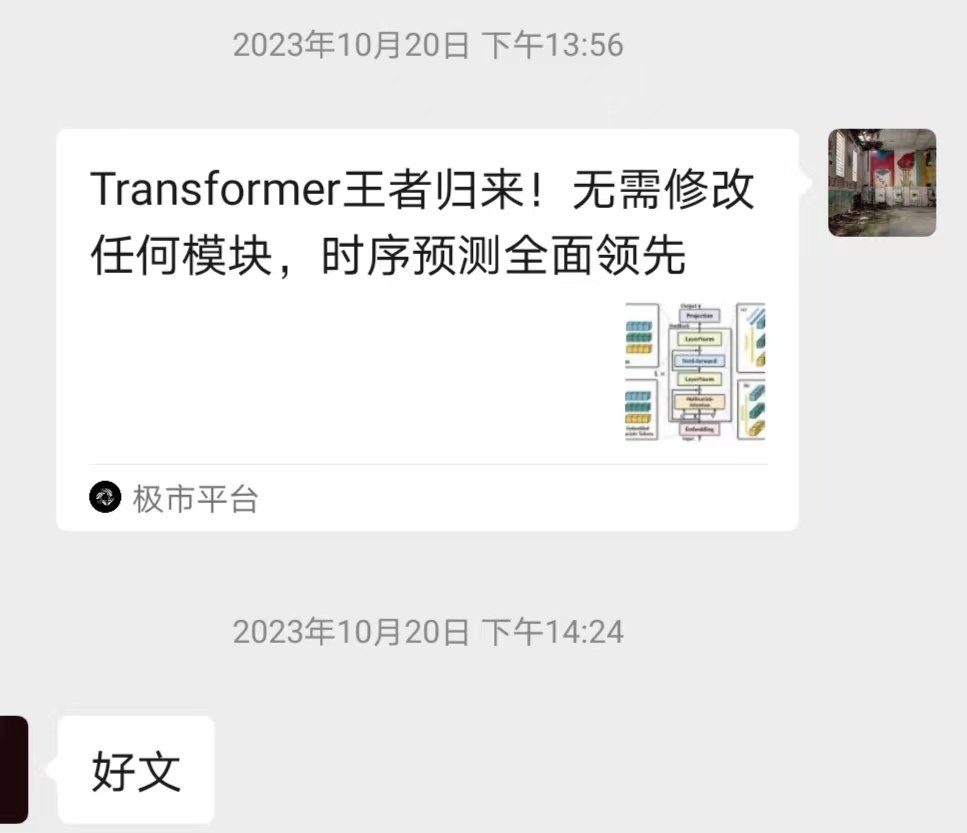
\includegraphics[width=0.5\textwidth]{./pic/itransformer_公众号.jpg}
  \caption{\small{2023年10月20日,我第一次在微信公众号接触到这篇文章}}
  \label{fig:wechat}
\end{figure}

正好这门课程的大作业就是复现论文,动工之前,我咨询了助教的意见,发现这是一篇在投的ICLR 2024的paper(毕竟论文还很新),不过已经在OpenReview上拿了3个8分和1个6分,基本确定能中,而且其官方仓库星星也很多,所以助教认为其符合顶会文章的作业要求,于是我也就决定了复现这篇论文。

这篇论文的官方实现还是十分优美的,在各种软件工程规范都遵守得很好,所以跑实验的过程中体验非常好,iTransformer的效果实际跑出来也非常不错。当然,体验没有那么好的一点就是深度学习的工作都要跑大量组别的实验,前前后后跑了接近八十组实验,在百度和kaggle的免费算力上跑了差不多40多个小时,有几回还是半夜挂机训练,终于跑出了上面那些规模庞大的表格。这让我提前体会到了未来在AI科研领域工作的艰辛。

十分感谢这次大作业的契机,让我得以经手这篇优美的工作,提升了我在实验方面的能力。同时也感谢这门课程,让我接触了深度学习各领域的优秀工作,大幅深化了我对深度学习的理解,提高了我的工程能力。

最后,感谢老师和助教的辛勤付出,祝老师和助教新年快乐,万事如意!


\bibliography{dllab_final_report}
\bibliographystyle{iclr2024_conference}

\vfill

\end{document}
